\documentclass[mathserif, aspectratio=169]{beamer}
\usetheme{odenpecos}
\setbeamertemplate{itemize/enumerate body begin}{\fontsize{8.8}{9}\selectfont}
\setbeamertemplate{itemize/enumerate subbody begin}{\fontsize{7.5}{8}\selectfont}
\setbeamertemplate{itemize/enumerate subsubbody begin}{\fontsize{7.5}{8}\selectfont}

% default search path for figures
\graphicspath{{./shared_figures/}{./figures/}}

\newcommand{\zapspace}{\topsep=0pt\partopsep=0pt\itemsep=0pt\parskip=0pt}

\usepackage{multicol}
\usepackage{pict2e}
\usepackage{esdiff}
\usepackage{multimedia}
\usepackage{verbatim}
\usepackage{mhchem}

\usepackage[percent]{overpic}
\usepackage[absolute,overlay]{textpos}

\newcommand{\overbar}[1]{\mkern 1.5mu\overline{\mkern-1.5mu#1\mkern-1.5mu}\mkern 1.5mu}
\newcommand{\pp}[2]{\frac{\partial #1}{\partial #2}}
\newcommand{\dd}[2]{\frac{d #1}{d #2}}
\newcommand{\DD}[2]{\frac{D #1}{D #2}}
\newcommand{\mm}{\mathbf{minmod}}
\def\etal{{\it et al~}}
\newcommand{\be}{\begin{eqnarray}}
\newcommand{\ee}{\end{eqnarray}}
\newcommand{\mbb}[1]{\mathbb{#1}} % math blackboard bold
\newcommand{\mcal}[1]{\mathcal{#1}} % math blackboard bold
\newcommand{\mbf}[1]{\mathbf{#1}} % math bold face (for vectors)
\newcommand{\sbf}[1]{\boldsymbol{#1}} % bold face for symbols
\newcommand{\jump}[1]{\llbracket #1 \rrbracket} % jump operator
\newcommand{\avg}[1]{\langle #1 \rangle} % average operator
\newcommand{\rarrow}{\rightarrow}
\newcommand{\Rarrow}{\Rightarrow}
\newcommand{\LRarrow}{\Leftrightarrow}
\newcommand{\vvvert}{|\kern-1pt|\kern-1pt|}
\newcommand{\enorm}[1]{\vvvert #1 \vvvert}
\newcommand{\nutil}{\tilde{\nu}}
\newcommand{\Var}{\mathrm{Var}}
\newcommand{\Cov}{\mathrm{Cov}}


\definecolor{MyDarkGreen}{rgb}{0,0.45,0.08}
\newcommand{\myred}[1]{{\color{red} #1}}
\newcommand{\myblue}[1]{{\color{blue} #1}}
\newcommand{\mygreen}[1]{{\color{MyDarkGreen} #1}}

\newcommand{\sa}{\nu_{\mathrm{sa}}}
\newcommand{\tep}{\tilde{\epsilon}}
\newcommand{\Ssd}{\mathcal{S}} % source term due to slow derivative
\newcommand{\ud}{\,\mathrm{d}}

\newcommand{\Mach}[1]{\ensuremath{\mbox{Ma}_{#1}}}
\newcommand{\Reynolds}{\ensuremath{\mathit{Re}}}
\newcommand{\DensityRat}{\ensuremath{\mathit{DR}}}
\newcommand{\BlowRat}{\ensuremath{\mbox{BR}}}
\newcommand{\VelRat}{\ensuremath{\mathit{VR}}}
\newcommand{\Tau}{\ensuremath{\mathrm{T}}}

\newcommand{\wall}     {\ensuremath{\mathrm{w}}}   % wall subindex
\newcommand{\awall}    {\ensuremath{\mathrm{aw}}}  % adiabatic wall subindex

\newcommand{\commentout}[1]{}

\newcommand{\vect}[1]{\boldsymbol{#1}}
\usepackage{mleftright}
\newcommand{\of}[1]{\mleft( #1 \mright)}
\newcommand{\vth}{v_{\textrm{th}}}
\newcommand{\reals}{\mathbb{R}}
\newcommand{\myint}[2]{\int\limits_{#1}^{#2}}

\DeclareMathOperator{\variance}{Var}

\begin{document}
% disable nav
\setbeamertemplate{navigation symbols}{}

% ---------------------------------------------------------------
% Oden/Pecos title page

\hoffset=.16in

\begin{frame}[plain,t]{}
\makeatletter
%\vspace*{0.85cm}
%\vspace*{0.65cm}
\includegraphics[height=0.9in,trim=50 40 40 0, clip]{PMSc_159_university_formal_horizontal.pdf} \newline
%\vspace*{0.3cm}
\begin{columns}[T,onlytextwidth]
\column{.8\textwidth}
{\bf \color{burntorange} \fontfamily{bch}\selectfont 
% -- Set talk title here
Solving the Boltzmann equation for electron kinetics using Petrov-Galerkin approach
% --
}
\end{columns}
\vspace*{.15cm}
\rule{.8\textwidth}{0.6pt} \newline

\vspace*{0.05cm}
\setstretch{0.65}
{\fontfamily{phv}\selectfont
  { \scriptsize
    % -- define presenter, authors here
    Milinda Fernando, Daniil Bochkov, Todd Oliver, George Biros\newline
    % --
  }
  {\color{burntorange} \tiny
    % -- define role, meeting event, location, etc
    Year-1 Review $\cdot$ August, 2021 $\cdot$ Austin, TX
    % --
  }
}

\vspace*{1cm}
%\includegraphics[height=0.3in]{figures/pecos_orange1.png}
\begin{columns}
\begin{column}{0.8\linewidth}
\includegraphics[height=0.5in]{oden_pecos_2020_wordmark.png}\\
{\scriptsize \url{https://pecos.oden.utexas.edu}}
\end{column}

\begin{column}{0.2\linewidth}
\includegraphics[height=0.6in]{psaap3-logo.png}
\end{column}
\end{columns}

\end{frame}
\hoffset=0in
% -- end title slide ---------------------------------------------

%===============================================================================
\begin{frame}
\frametitle{Boltzmann equation}
%
\begin{itemize}
\item \textbf{Importance:} 
%Electron density function $f_e = f_e(\vect{x}, \vect{v}, t)$ defines transport and kinetic properties
Distribution function of electrons defines transport and kinetic properties
\\
$\rightarrow$ Need to couple plasma model with electron kinetics (Y3)
\item Evolution of $f_e = f_e(\vect{x}, \vect{v}, t)$ obeys the \textbf{Boltzmann equation}
\small
\begin{align*}
\partial_t f_e + \vect{v}\cdot \nabla_{\vect{x}} f_e  + \vect{L} \cdot \nabla_{\vect{v }}f_e = \sum_{a} C_a(f_e)
\end{align*}
where, for example, in case of $a=$ elastic collisions
\begin{align*}
C_a(f_e) &= n_0\int_{S^2} v \underbrace{\sigma_a(v,\omega)}_{\tiny\text{\tiny scat. cross sec.}} 
\left( f_e(v^\prime) - f_e(v) \right) \ud \omega 
\end{align*}
\item \textbf{Main challenge}: 6+1 dimensions
\item \textbf{Idea}: FEM in $\vect{x}$, spectral in $\vect{v}$
\item \textbf{Currently (Y1)}: spatially homogeneous case $f_e = f_e(\vect{v}, t)$ to investigate efficient velocity-space discretizations
\begin{align*}
\partial_t f_e = \sum_{a} C_a(f_e)
\end{align*}
\end{itemize}
%
\end{frame}
%
%\begin{frame}
%\frametitle{Boltzmann equation}
%%
%Boltzmann equation for electron-heavy neutral collisions can be modeled by, 
%\begin{itemize}
%\item Electron density function $f_e = f_e(\vect{x}, \vect{v}, t)$
%\end{itemize}
%\small
%\begin{align*}
%\partial_t f_e + \vect{v}\cdot \nabla_{\vect{x}} f_e  + \vect{L} \cdot \nabla_{\vect{v }}f_e = Q(f_e)
%\end{align*}
%where, for example, for a given collision $a$
%\begin{align*}
%Q_a(f_e) &= n_0\int_{S^2} v \sigma_a(v,\omega) 
%\left( f(v^\prime) - f(v) \right) d\omega \text{ where } Q(f_e) = \sum_{a} Q_a(f_e)
%\end{align*}
%% \item \textbf{Main challenge}: 6+1 dimensions
%% \item \textbf{Idea}: FEM in $\vect{x}$, spectral in $\vect{v}$
%% \item \textbf{So far}: spatially homogeneous case $f = f(\vect{v}, t)$ to ensure efficiency of velocity-space discretization
%% \begin{align*}
%% \partial_t f = Q(f,f)
%% \end{align*}
%% \end{itemize}
%%
%\end{frame}
%
%\begin{frame}{Challenges}
%  \begin{itemize}
%  \item \textbf{Dimensionality}  : Boltzmann equation is a 7d problem. 
%  \item \textbf{Numerical methods} : Numerical method to use ? What basis expansions are best to use ?
%  \item \textbf{Collision integral} : 5d integral evaluation. 
%  \item \textbf{HPC challenges} : Parallelization, performance portability ... 
%  %\item \textbf{Parallelization} : Efficient parallelization of the problem (i.e., partitioning challenges) specially in adaptive discretization environment. 
%  \end{itemize}
%  \ \\ \ \\ \ \\
%\textbf{Currently working}: Solving the collision operator, i.e., 
%\begin{align*}
%\partial_t f_e = Q(f_e)
%\end{align*}
%\end{frame}

%===============================================================================
\begin{frame}
\frametitle{Petrov-Galerkin approach}
%
\small
\begin{itemize}

\item Weak formulation:
$
\displaystyle
\quad
\partial_t f = Q(f,f)
\quad \rightarrow \quad
\partial_t \myint{R^3}{} f \phi\of{\vect{v}} \ud \vect{v} =
\myint{R^3}{} Q(f) \phi\of{\vect{v}} \ud \vect{v}
$

\item Solution as a perturbed Maxwellian:
\begin{align*}
f\of{\vect{v}} = M\of{v} h\of{\vect{v},t}
, \quad\quad
%M\of{v} = \frac{n}{\left( \vth \sqrt{\pi} \right)^3} e^{-\left(\frac{v}{\vth}\right)^2}
M\of{v} = n_e \left( \frac{m}{2 \pi kT }\right)^{\frac32} e^{-\frac{mv^2}{2kT}}
%, \quad
%\vth = \sqrt{\frac{2kT}{m}}
\end{align*}

\item Expansion in basis functions:
\begin{align*}
h\of{\vect{v},t} =
\sum_{k,l,m} h_{k,l,m} \of{t} \Phi_k\of{v} \underbrace{Y_{lm}\of{v_\theta, v_\phi}}_{\tiny\text{sph. harm.}},
\quad
\quad
\phi\of{\vect{v}} = \Phi_p\of{v} \underbrace{Y_{qs}\of{v_\theta, v_\phi}}_{\tiny\text{sph. harm.}}
\end{align*}

\item Resulting system of ODEs:
\begin{align*}
\sum_{k,l,m} M_{p,q,s}^{k,l,m} \partial_t h_{k,l,m}\of{t} = \sum_{k,l,m}  L_{p,q,s}^{k,l,m} h_{k,l,m}\of{t}
\end{align*}
\end{itemize}
%
\end{frame}

%===============================================================================
\begin{frame}
\frametitle{Investigation of different bases}
%
\begin{itemize}
\item Choice of basis functions in radial direction
\end{itemize}
\small
\begin{align*}
\textrm{Assoc. Laguerre poly:}
& \quad \Phi_n\of{v} = L_n\of{v^2}, &&
\quad 
\myint{0}{+\infty} v^2 e^{-v^2} L_n\of{v^2} L_{n^\prime}\of{v^2} \ud v \sim \delta_{nn^\prime}
\\
\textrm{Maxwell (speed) poly:}
& \quad \Phi_n\of{v} = P_n\of{v}, &&
\quad 
\myint{0}{+\infty} v^2 e^{-v^2} P_n\of{v} P_{n^\prime}\of{v} \ud v \sim \delta_{nn^\prime}
\\
\textrm{Chebyshev poly:}
& \quad \Phi_n\of{v} = C_n\of{v}, &&
\quad 
\myint{-1}{1} \left(1-v^2\right)^{-\frac12} C_n\of{v} C_{n^\prime}\of{v} \ud v \sim \delta_{nn^\prime}
\\
\textrm{Linear interp:}
& \quad \Phi_n\of{v} = N_n\of{v}, &&
\quad 
N_n\of{v} = 1 - \frac{|x-x_n|}{\Delta x},\quad x_{n-1} < x < x_{n+1}
\end{align*}

%\begin{columns}
%\begin{column}{0.6\linewidth}
%\begin{itemize}
%\item Geometry non-dimensionalized by coil radius
%\item Coil approximated by square rings
%\item $\Omega = (0, R) \times (0, H)$, $R = 2.8$, $H=6.4$
%\item Grid: $154 \times 76 = 11704$ quads
%\item $h = 0.025$ near coils
%\item Colors on right indicate coil locations
%\end{itemize}
%\end{column}
%\begin{column}{0.4\linewidth}
%  \vspace{-0.75in}
%  \begin{center}
%    \includegraphics[height=8.2cm]{example-image-a}
%  \end{center}
%\end{column}
%\end{columns}
%
\end{frame}

%===============================================================================
\begin{frame}
\frametitle{Investigation of different bases}
%
\begin{columns}[T]
\begin{column}{0.3\linewidth}
\begin{itemize}
\item Bolsig+ data for Ar 
\item Included reactions:
\hspace{-0.5in}
\begin{itemize}
\item Elastic: $e + \text{Ar} \rightarrow e + \text{Ar}$
\item Excitation: $e + \text{Ar} \rightarrow e + \text{Ar}^*$
\item Ionization: $e + \text{Ar} \rightarrow e + \text{Ar}^+ + e$
\end{itemize}
\item Electric field $E/N$:
\begin{itemize}
\item $1\times 10^{-26}\, \text{V} \cdot \text{m}^2$
\item $1\times 10^{-24}\, \text{V} \cdot \text{m}^2$
\item $7\times 10^{-24}\, \text{V} \cdot \text{m}^2$
\item $1\times 10^{-23}\, \text{V} \cdot \text{m}^2$
\item $6\times 10^{-19}\, \text{V} \cdot \text{m}^2$
\end{itemize}
\end{itemize}
\end{column}
\begin{column}{0.7\linewidth}
  \vspace{-0.35in}
  \begin{center}
   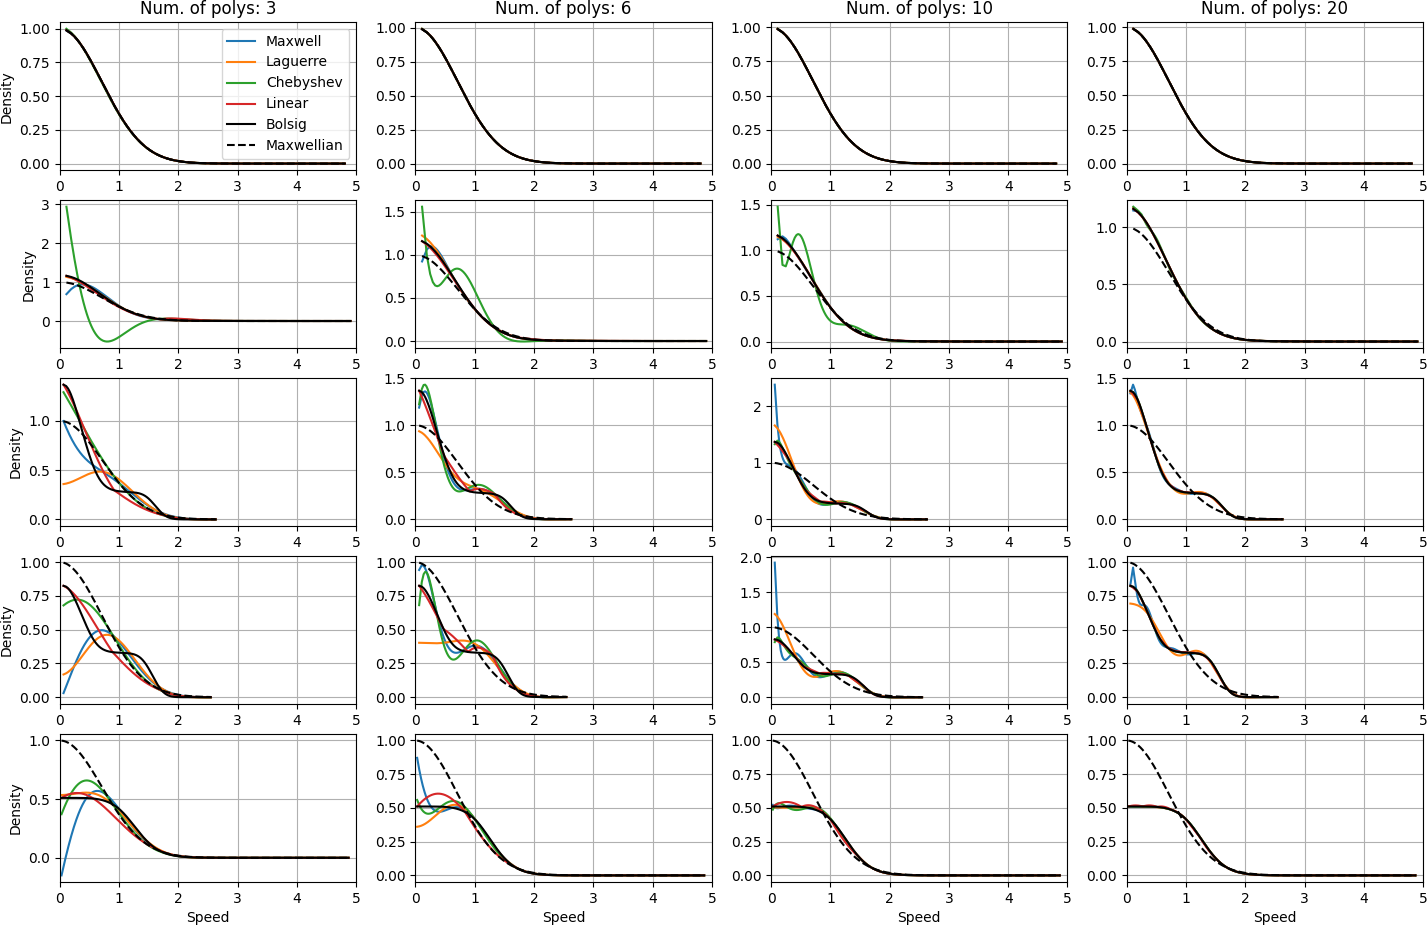
\includegraphics[width=\textwidth]{figures/bolsig_visual_lin.png}
  \end{center}
\end{column}
\end{columns}
%
\end{frame}

%===============================================================================
\begin{frame}
\frametitle{Investigation of different bases}
%
\begin{columns}[T]
\begin{column}{0.3\linewidth}
\begin{itemize}
\item Bolsig+ data for Ar 
\item Included reactions:
\begin{itemize}
\item Elastic: $e + \text{Ar} \rightarrow e + \text{Ar}$
\item Excitation: $e + \text{Ar} \rightarrow e + \text{Ar}^*$
\item Ionization: $e + \text{Ar} \rightarrow e + \text{Ar}^+ + e$
\end{itemize}
\item Electric field $E/N$:
\begin{itemize}
\item $1\times 10^{-26}\, \text{V} \cdot \text{m}^2$
\item $1\times 10^{-24}\, \text{V} \cdot \text{m}^2$
\item $7\times 10^{-24}\, \text{V} \cdot \text{m}^2$
\item $1\times 10^{-23}\, \text{V} \cdot \text{m}^2$
\item $6\times 10^{-19}\, \text{V} \cdot \text{m}^2$
\end{itemize}
\end{itemize}
\end{column}
\begin{column}{0.7\linewidth}
  \vspace{-0.35in}
  \begin{center}
   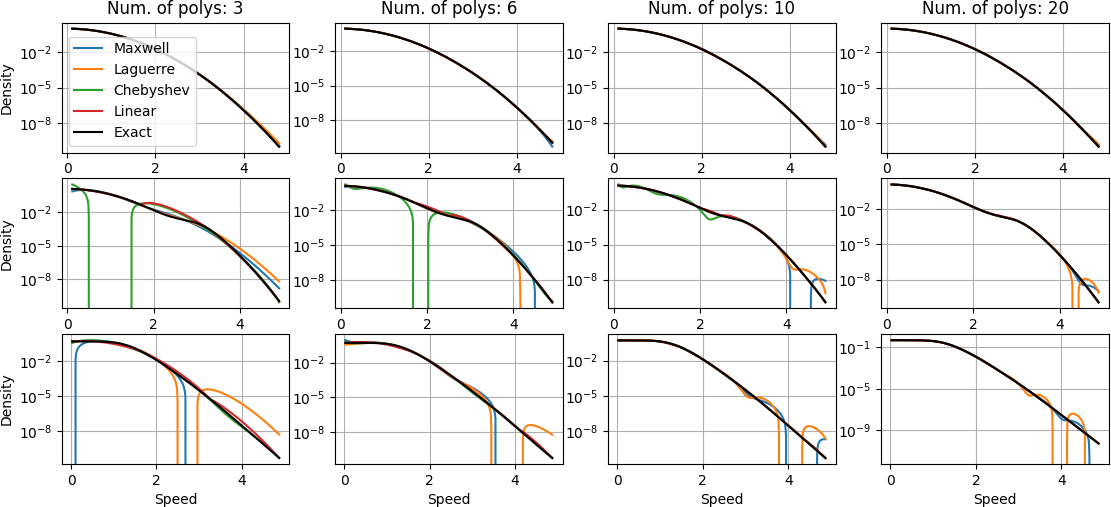
\includegraphics[width=\textwidth]{figures/bolsig_visual.png}
  \end{center}
\end{column}
\end{columns}
%
\end{frame}

%===============================================================================
\begin{frame}
\frametitle{Investigation of different bases}
%
\begin{columns}[T]
\begin{column}{0.3\linewidth}
\begin{itemize}
\item Error measures
\begin{itemize}
\item EDF $f$ itself: $L_\infty$, $L_2$
\item Reaction rate
$k_a = \gamma \int \varepsilon \sigma_a f \ud \varepsilon$
where 
\\$a=$ elastic, excitation, collision
\end{itemize}
\item Takeaways:
\begin{itemize}
\item No obvious choice
\item Needs further investigation
\end{itemize}
\end{itemize}
\end{column}
\begin{column}{0.7\linewidth}
  \vspace{-0.35in}
  \begin{center}
   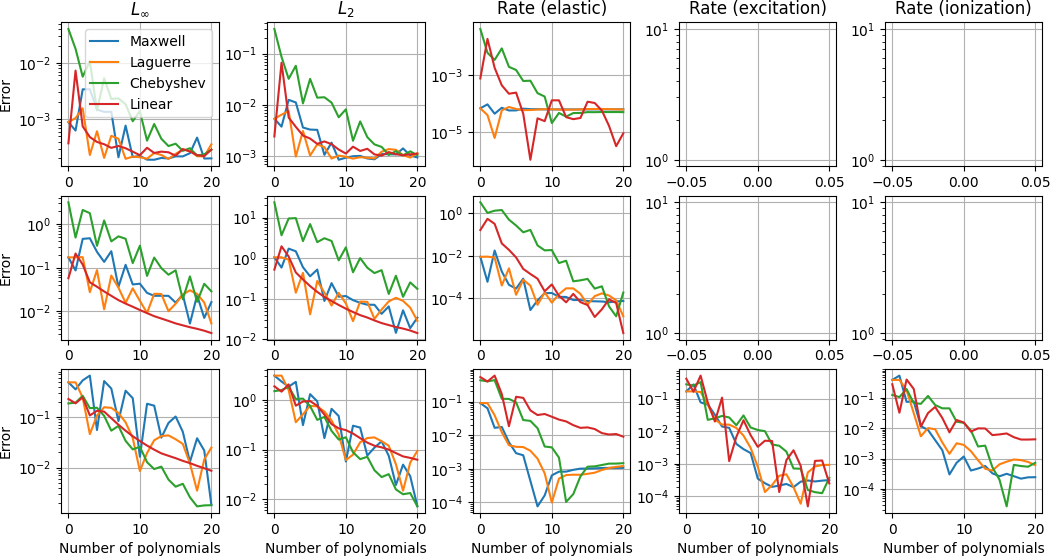
\includegraphics[width=\textwidth]{figures/bolsig_convergence.png}
  \end{center}
\end{column}
\end{columns}
%
\end{frame}


%===============================================================================

\begin{frame}
\frametitle{Solver implementation}
%
\begin{columns}[T]
\begin{column}{0.6\linewidth}
\begin{itemize}
\item Python 
\item 5-dimensional integrations: 
\begin{itemize}
\item Tenzorized implementation
\item 0.0093s vs 5.2256s loop-based
\end{itemize}
\item Flexible choice of basis functions in radial directions
\item Reactions implemented
\begin{itemize}
\item Elastic: $e + \text{Ar} \rightarrow e + \text{Ar}$
\item Excitation: $e + \text{Ar} \rightarrow e + \text{Ar}^*$
\item Ionization: $e + \text{Ar} \rightarrow e + \text{Ar}^+ + e$
\end{itemize}
\item Currently: testing and verification
\end{itemize}
\end{column}
\begin{column}{0.4\linewidth}
  \vspace{-0.35in}
  \begin{center}
   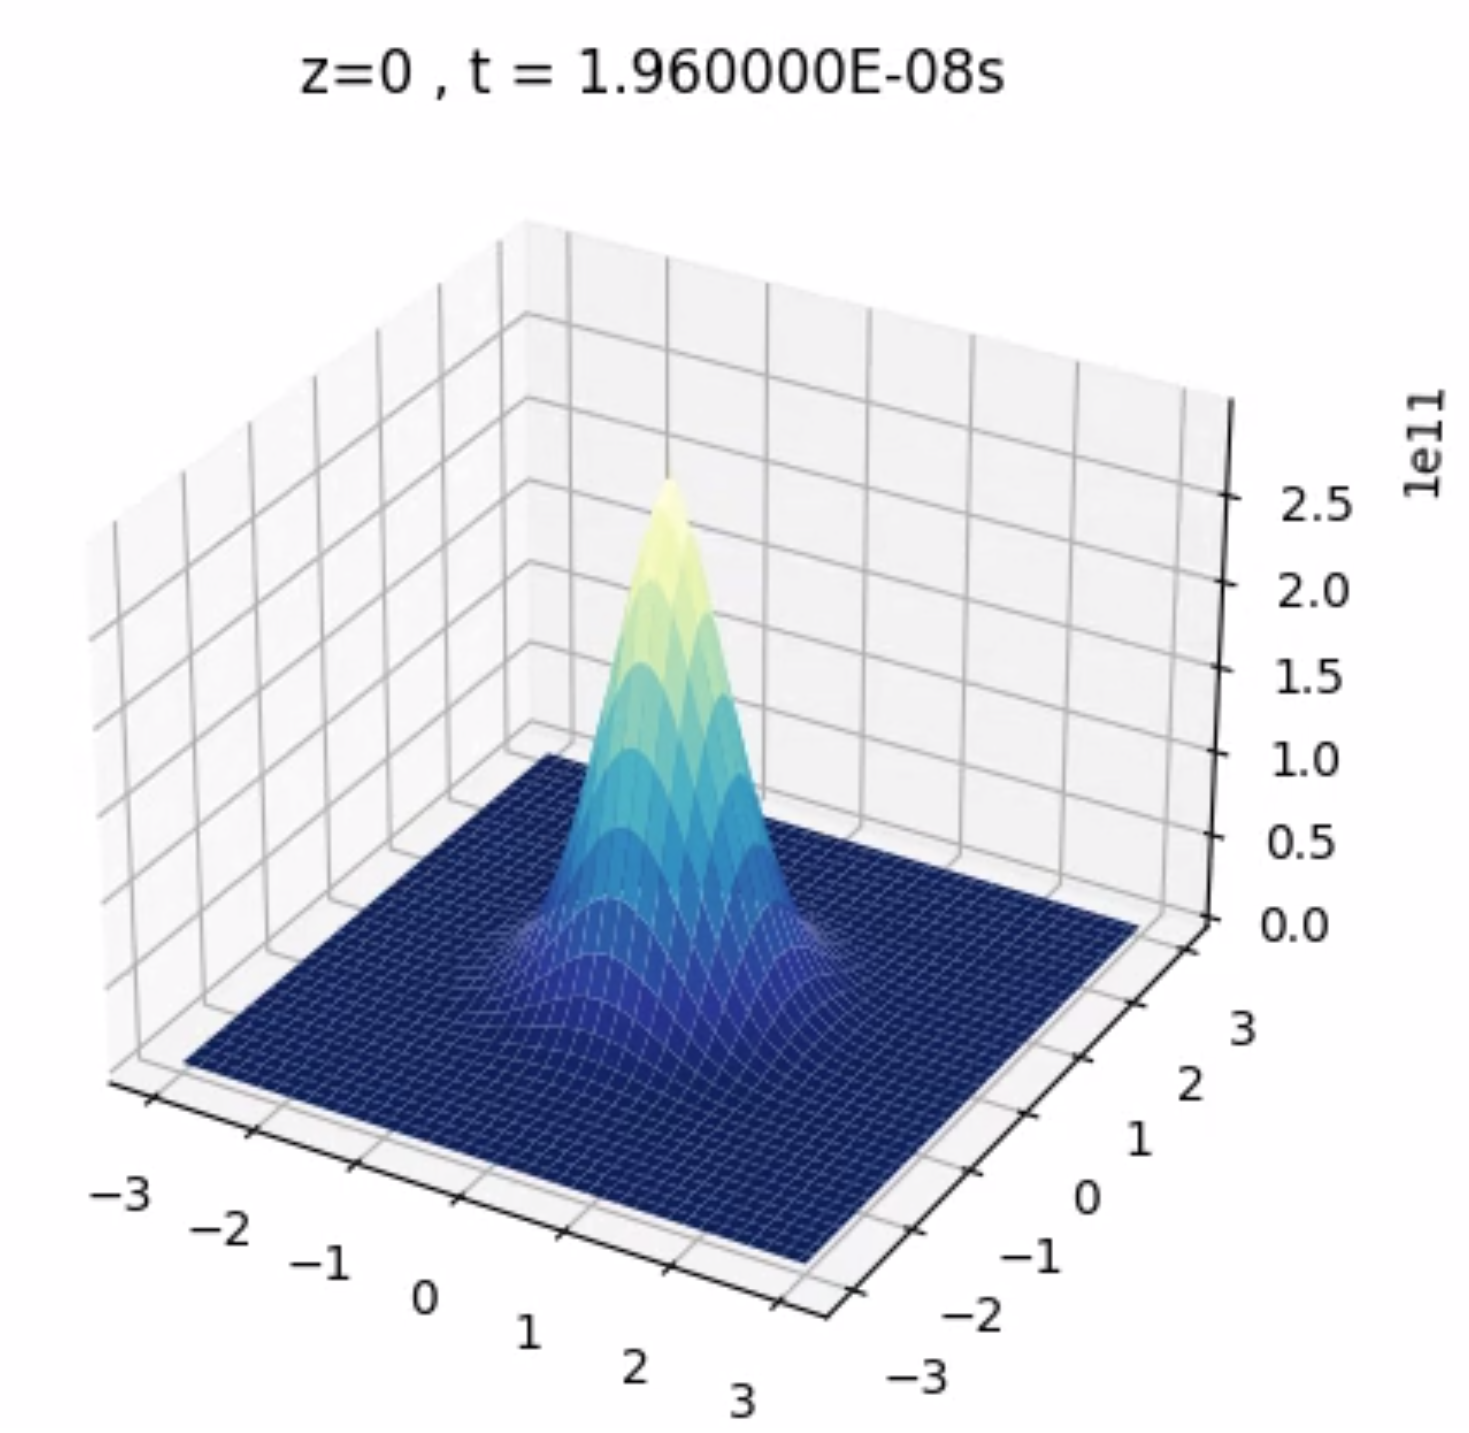
\includegraphics[width=\textwidth]{figures/code.png}
  \end{center}
\end{column}
\end{columns}
%
\end{frame}


%===============================================================================
\end{document}

